\documentclass[twoside]{book}

% Packages required by doxygen
\usepackage{fixltx2e}
\usepackage{calc}
\usepackage{doxygen}
\usepackage[export]{adjustbox} % also loads graphicx
\usepackage{graphicx}
\usepackage[utf8]{inputenc}
\usepackage{makeidx}
\usepackage{multicol}
\usepackage{multirow}
\PassOptionsToPackage{warn}{textcomp}
\usepackage{textcomp}
\usepackage[nointegrals]{wasysym}
\usepackage[table]{xcolor}

% Font selection
\usepackage[T1]{fontenc}
\usepackage[scaled=.90]{helvet}
\usepackage{courier}
\usepackage{amssymb}
\usepackage{sectsty}
\renewcommand{\familydefault}{\sfdefault}
\allsectionsfont{%
  \fontseries{bc}\selectfont%
  \color{darkgray}%
}
\renewcommand{\DoxyLabelFont}{%
  \fontseries{bc}\selectfont%
  \color{darkgray}%
}
\newcommand{\+}{\discretionary{\mbox{\scriptsize$\hookleftarrow$}}{}{}}

% Page & text layout
\usepackage{geometry}
\geometry{%
  a4paper,%
  top=2.5cm,%
  bottom=2.5cm,%
  left=2.5cm,%
  right=2.5cm%
}
\tolerance=750
\hfuzz=15pt
\hbadness=750
\setlength{\emergencystretch}{15pt}
\setlength{\parindent}{0cm}
\setlength{\parskip}{3ex plus 2ex minus 2ex}
\makeatletter
\renewcommand{\paragraph}{%
  \@startsection{paragraph}{4}{0ex}{-1.0ex}{1.0ex}{%
    \normalfont\normalsize\bfseries\SS@parafont%
  }%
}
\renewcommand{\subparagraph}{%
  \@startsection{subparagraph}{5}{0ex}{-1.0ex}{1.0ex}{%
    \normalfont\normalsize\bfseries\SS@subparafont%
  }%
}
\makeatother

% Headers & footers
\usepackage{fancyhdr}
\pagestyle{fancyplain}
\fancyhead[LE]{\fancyplain{}{\bfseries\thepage}}
\fancyhead[CE]{\fancyplain{}{}}
\fancyhead[RE]{\fancyplain{}{\bfseries\leftmark}}
\fancyhead[LO]{\fancyplain{}{\bfseries\rightmark}}
\fancyhead[CO]{\fancyplain{}{}}
\fancyhead[RO]{\fancyplain{}{\bfseries\thepage}}
\fancyfoot[LE]{\fancyplain{}{}}
\fancyfoot[CE]{\fancyplain{}{}}
\fancyfoot[RE]{\fancyplain{}{\bfseries\scriptsize Generated by Doxygen }}
\fancyfoot[LO]{\fancyplain{}{\bfseries\scriptsize Generated by Doxygen }}
\fancyfoot[CO]{\fancyplain{}{}}
\fancyfoot[RO]{\fancyplain{}{}}
\renewcommand{\footrulewidth}{0.4pt}
\renewcommand{\chaptermark}[1]{%
  \markboth{#1}{}%
}
\renewcommand{\sectionmark}[1]{%
  \markright{\thesection\ #1}%
}

% Indices & bibliography
\usepackage{natbib}
\usepackage[titles]{tocloft}
\setcounter{tocdepth}{3}
\setcounter{secnumdepth}{5}
\makeindex

% Hyperlinks (required, but should be loaded last)
\usepackage{ifpdf}
\ifpdf
  \usepackage[pdftex,pagebackref=true]{hyperref}
\else
  \usepackage[ps2pdf,pagebackref=true]{hyperref}
\fi
\hypersetup{%
  colorlinks=true,%
  linkcolor=blue,%
  citecolor=blue,%
  unicode%
}

% Custom commands
\newcommand{\clearemptydoublepage}{%
  \newpage{\pagestyle{empty}\cleardoublepage}%
}

\usepackage{caption}
\captionsetup{labelsep=space,justification=centering,font={bf},singlelinecheck=off,skip=4pt,position=top}

%===== C O N T E N T S =====

\begin{document}

% Titlepage & ToC
\hypersetup{pageanchor=false,
             bookmarksnumbered=true,
             pdfencoding=unicode
            }
\pagenumbering{alph}
\begin{titlepage}
\vspace*{7cm}
\begin{center}%
{\Large My Project }\\
\vspace*{1cm}
{\large Generated by Doxygen 1.8.13}\\
\end{center}
\end{titlepage}
\clearemptydoublepage
\pagenumbering{roman}
\tableofcontents
\clearemptydoublepage
\pagenumbering{arabic}
\hypersetup{pageanchor=true}

%--- Begin generated contents ---
\chapter{Simulador Sistemas Embebidos Robotino}
\label{index}\hypertarget{index}{}\hypertarget{index_autotoc_md0}{}\section{Overview}\label{index_autotoc_md0}
Esta es la documentación del proyecto final de la catedra de Programación Orientada a Objetos en C++.\hypertarget{index_autotoc_md1}{}\section{Objetivos}\label{index_autotoc_md1}


El objetivo es simular la comunicación de 2 arduinos y una raspberry. Ademas, en la raspberry hay un thread corriendo que representa a una camara y envia datos de posición a la raspberry.\hypertarget{index_autotoc_md2}{}\section{Caracteristicas de los SE}\label{index_autotoc_md2}
\hypertarget{index_autotoc_md3}{}\subsection{Raspberry}\label{index_autotoc_md3}

\begin{DoxyItemize}
\item Intercambia mensajes con los Arduinos\+: Recibe mediciones de I\+MU y sensor de distancia y envia seteo de la bomba de agua.
\item Recibe datos del thread de la camara
\end{DoxyItemize}\hypertarget{index_autotoc_md4}{}\subsection{Arduino R}\label{index_autotoc_md4}

\begin{DoxyItemize}
\item Posee una I\+MU que mide aceleraciones en 3 ejes
\item Tiene conectada una bomba de agua a la cual se le setea la tensión
\end{DoxyItemize}\hypertarget{index_autotoc_md5}{}\subsection{Arduino L}\label{index_autotoc_md5}

\begin{DoxyItemize}
\item Tiene un sensor de posición laser
\end{DoxyItemize}\hypertarget{index_autotoc_md6}{}\section{Esquema del programa}\label{index_autotoc_md6}
El programa principal es el archivo \hyperlink{main_8cpp}{main.\+cpp}, donde se disparan los siguientes threads\+:
\begin{DoxyItemize}
\item AR\+: Corre el programa princiapl del Arduino R. En el se toman datos de una I\+MU y se envian a la raspberry. Ademas se leen mensajes que provienen de la raspberry para setear actuadores.
\item AL\+: Corre el programa principal del Arduino L. En el mismo se toman datos de un sensor de distancia y se envian a la raspberry
\item R\+PI\+: Corre el thread de la raspberry pi, dentro del cual se corren lo siguientes threads\+:
\begin{DoxyItemize}
\item Main\+: Corre el programa principal de la raspi, en el mismo se leen datos que provienen de los arduinos y se envian datos para setear los actuadores.
\item Camara\+: Lee datos de posición de la camara y los envia al programa principal de la raspi
\end{DoxyItemize}
\item Quit\+: Revisa si el usuario quiere terminar la simulacion (enter) en caso de querer terminar cierra todos los threads.
\end{DoxyItemize}

Para la generación de los datos de la I\+MU y la camara se leen archivos .txt con los datos de aceleración y posición. En el caso del sensor de distancia, se generan numeros aleatorios para representar la posición medida.\hypertarget{index_autotoc_md7}{}\section{Comunicaciones}\label{index_autotoc_md7}
Para simular la comunicación utilizo queue con strings como elementos donde voy metiendo los mensajes que quiero mandar a otros dispositivos, y el otro dispositivo lee si le corresponde y si le corresponde lo pop, sino no hace nada.

Las siguientes queue se utilizan\+:
\begin{DoxyItemize}
\item queue 1\+: Comunicación entre los arduinos y raspi
\item queue 2\+: Comunicación entre la raspi y la camara
\end{DoxyItemize}\hypertarget{index_autotoc_md8}{}\subsection{Envio de datos}\label{index_autotoc_md8}
A continuación se muestra la estructura de los mensajes de cada dispositivo. \subsubsection*{I\+MU}

!\+D\+AT\+:I\+M\+U\+:xxxx\+:yyyy\+:zzzz\+:\#

\subsubsection*{C\+A\+M\+E\+RA}

!\+D\+AT\+:C\+A\+M\+:xxxx\+:yyyy\+:zzzz\+:\#

\subsubsection*{L\+A\+S\+ER}

!\+D\+AT\+:L\+A\+S\+:xxxx\+:\# 
\chapter{Class Index}
\section{Class List}
Here are the classes, structs, unions and interfaces with brief descriptions\+:\begin{DoxyCompactList}
\item\contentsline{section}{\hyperlink{classhello}{hello} \\*Simple brief intro  detailed intro }{\pageref{classhello}}{}
\end{DoxyCompactList}

\chapter{File Index}
\section{File List}
Here is a list of all documented files with brief descriptions\+:\begin{DoxyCompactList}
\item\contentsline{section}{\hyperlink{main_8cpp}{main.\+cpp} }{\pageref{main_8cpp}}{}
\item\contentsline{section}{\hyperlink{robsim_8h}{robsim.\+h} }{\pageref{robsim_8h}}{}
\end{DoxyCompactList}

\chapter{Class Documentation}
\hypertarget{classhello}{}\section{hello Class Reference}
\label{classhello}\index{hello@{hello}}


simple brief intro  detailed intro  


\subsection*{Public Member Functions}
\begin{DoxyCompactItemize}
\item 
\mbox{\Hypertarget{classhello_a7fabfcda038de9dd88bff7f4c3bf704d}\label{classhello_a7fabfcda038de9dd88bff7f4c3bf704d}} 
void \hyperlink{classhello_a7fabfcda038de9dd88bff7f4c3bf704d}{helloworld} ()
\begin{DoxyCompactList}\small\item\em print helloworld on the terminal \end{DoxyCompactList}\end{DoxyCompactItemize}


\subsection{Detailed Description}
simple brief intro  detailed intro 

The documentation for this class was generated from the following file\+:\begin{DoxyCompactItemize}
\item 
\hyperlink{helloworld_8cc}{helloworld.\+cc}\end{DoxyCompactItemize}

\chapter{File Documentation}
\hypertarget{helloworld_8cc}{}\section{helloworld.\+cc File Reference}
\label{helloworld_8cc}\index{helloworld.\+cc@{helloworld.\+cc}}


helloworld  this is a simple hello world program using a function  


{\ttfamily \#include $<$iostream$>$}\newline
Include dependency graph for helloworld.\+cc\+:\nopagebreak
\begin{figure}[H]
\begin{center}
\leavevmode
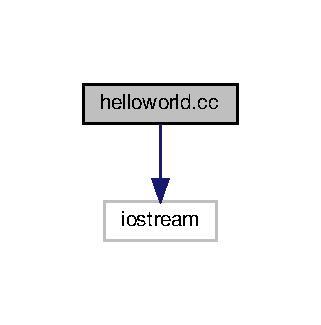
\includegraphics[width=154pt]{helloworld_8cc__incl}
\end{center}
\end{figure}
\subsection*{Classes}
\begin{DoxyCompactItemize}
\item 
class \hyperlink{classhello}{hello}
\begin{DoxyCompactList}\small\item\em simple brief intro  detailed intro \end{DoxyCompactList}\end{DoxyCompactItemize}
\subsection*{Functions}
\begin{DoxyCompactItemize}
\item 
\mbox{\Hypertarget{helloworld_8cc_ae66f6b31b5ad750f1fe042a706a4e3d4}\label{helloworld_8cc_ae66f6b31b5ad750f1fe042a706a4e3d4}} 
int {\bfseries main} ()
\end{DoxyCompactItemize}


\subsection{Detailed Description}
helloworld  this is a simple hello world program using a function 

\begin{DoxyAuthor}{Author}
Francisco Ortiz 
\begin{DoxyCodeInclude}
\end{DoxyCodeInclude}
 
\end{DoxyAuthor}

%--- End generated contents ---

% Index
\backmatter
\newpage
\phantomsection
\clearemptydoublepage
\addcontentsline{toc}{chapter}{Index}
\printindex

\end{document}
